\documentclass[paper=a4,fontsize=12pt,parskip=half]{scrartcl}

%% packages
\usepackage[ngerman]{babel}
\usepackage{fontspec}
\usepackage{lmodern}
\usepackage{color}
\usepackage{graphicx}
\usepackage[autostyle=true,german=quotes]{csquotes}
\usepackage[hidelinks=true,colorlinks=false]{hyperref}
\usepackage{listings}

\definecolor{darkgray}{rgb}{.2,.2,.2}

\lstset{basicstyle=\footnotesize\ttfamily,breaklines=true}

\lstdefinelanguage{Grammar}{
  keywords={grammar, typedef, node, prop, terminal, children},
  keywordstyle=\color{blue},
  ndkeywords={string, boolean, between, allowed, sequence},
  ndkeywordstyle=\color{black},
  identifierstyle=\color{black},
  sensitive=false,
  commentstyle=\color{purple}\ttfamily,
  stringstyle=\color{red}\ttfamily,
  morestring=[b]',
  morestring=[b]"
}

\hypersetup{
  pdftitle={Generierung von syntaxfreien Programmierumgebungen für beliebige Programmiersprachen},
  pdfsubject={Bewerbung um einen Stipendienplatz},
  pdfauthor={Marcus Riemer}
}

\usepackage[backend=biber,defernumbers=true,sorting=none]{biblatex}
\addbibresource[datatype=bibtex]{diss.bib}

\begin{document}

\section{Generierung von syntaxfreien Editoren für beliebige Programmiersprachen}

Konventionelle Entwicklungsumgebungen sind speziell auf die Bedürfnisse von professionellen Anwendern zugeschnittene Programme welche sich, aufgrund der damit verbundenen Komplexität, aus didaktischer Sicht nur eingeschränkt für die Einführung in die Programmierung eignen. Im Rahmen der Promotion soll erforscht und praktisch demonstriert werden, wie sich aus formalen Beschreibung von Programmiersprachen benutzerfreundliche, syntaxfreie Editoren speziell für Lernende erzeugen lassen können.

Abbildung~\ref{fig:example-sql-ide} zeigt ein Beispiel für einen solchen generierten Editor. Die Konzeption dieser generierten Editor-Umgebungen orientiert sich an den Erfahrungen, welche die Forscher hinter Projekten wie Scratch \cite{resnick_scratch:_2009} oder Googles Blockly gemacht haben \cite{fraser_ten_2015}.

\lstinputlisting[float=p,label={lst:partial-sql-grammar},caption={Auszug aus der Grammatik für SQL},captionpos=b,language={Grammar}]{sql.grammar}

\begin{figure}[p]
  \includegraphics[width=\linewidth]{screenshot-drag-drop-ide.png}
  \caption{Generierte Umgebung für die Programmiersprache \texttt{SQL}}
  \label{fig:example-sql-ide}
\end{figure}

Bei den als Eingabe fungierenden formalen Beschreibungen handelt es sich um eine noch nicht endgültig spezifizierte Abwandlung \enquote{typischer} Grammatiken wie sie zur Definition der Syntax in fast jedem Compiler zum Einsatz kommen \cite[S. 42ff]{aho_compilers:_2007}. Generell sind Ergänzungen und Abwandlungen notwendig, da die gängige rein syntax-orientierte Sichtweise für die Übersetzung in eine grafische Oberfläche keinerlei Informationen über die Darstellung enthält. Listing~\ref{lst:partial-sql-grammar} illustriert die Struktur dieser Grammatiken anhand eines Auszuges aus einer Grammatik für \texttt{SQL}. Die in Abbildung~\ref{fig:example-sql-ide} zu sehenden Farbstile wurden auf Basis von Eigenschaften wie \texttt{"keyword"} vergeben.

Die automatisierte Übersetzung der Grammatiken ermöglicht es erfahrenen Anwendern, zum Beispiel Lehrkräften, gegebene Programmiersprachen didaktisch motiviert einzuschränken. So wäre es zum Beispiel mögliche eine Variante von \texttt{SQL} zu erstellen, bei welcher die \texttt{GROUP BY}-Komponente nicht zur Verfügung steht. In Anlehnung an die bei \cite{klaeren_macht_2007} beschriebenen \enquote{Sprachebenen} soll sich so der Funktionsumfang der generierten Entwicklungsumgebungen an den Lernfortschritt der Klassengemeinschaft anpassen.

Die automatisch generierten Editoren sollen zudem kontextsensitive Unterstützung beim Programmieren anbieten. Da alle Manipulationen durch den Benutzer immer auf einem Syntaxbaum stattfinden, können auch bei unvollständigen (Teil-)Programmen typisierte Löcher (entlehnt aus Sprachen wie Haskell \cite{jones_haskell_2014}) genutzt werden, um die Menge an verfügbaren Operationen zu limitieren oder bestimmte Operationen hervorzuheben.

Zusammengefasst sollen also folgende Aspekte erforscht und demonstriert werden, ...

\begin{itemize}
\item wie auf Basis der beschriebenen Verfahren Editoren für unterschiedliche Klassen von Programmiersprachen generieren lassen.
\item welche zusätzlichen Annotationen für Grammatiken sinnvoll und notwendig sind, um mit den generierten Oberflächen Lernenden einen möglichst intuitiven Zugang zur Programmierung zu ermöglichen.
\item wie sich für Lernende automatisiert kontextabhängige Hinweise zur korrekten Vervollständigung der Programme geben lassen können.
\end{itemize}


\section{Detaillierte Konzeption}

Ein zentraler Aspekt des Vorhabens liegt in der Aufteilung auf theoretische und praktische Anteile: Die im Rahmen der Arbeit zu treffenden Annahmen sollen durch die praktische Implementierung bestmöglich verifiziert werden. Das Projekt befindet sich damit in einem etwas ungewöhnlichen Spannungsfeld zwischen der klassischen Informatik-Kerndisziplin \enquote{Übersetzerkonstruktion} (\enquote{Compilerbau}) und der Informatik-Didaktik. Darüber hinaus spielen auch Aspekte der Mensch-Computer-Interaktion eine Rolle, schließlich geht es neben der Verifikation der Programme auch um die Konstruktion benutzerfreundlicher Schnittstellen.

Um die einfachste Verwendung der Software für Lernende zu gewährleisten, wird das Projekt als Webanwendung entwickelt. Für die ersten Schritte der Softwareentwicklung reicht auf Seiten der Lernenden dann ein beliebiger, aktueller Browser. Mit diesem Ansatz in guter Gesellschaft: Das \enquote{große Vorbild} Scratch ist ebenfalls über den Browser erreichbar, genau so wie auch die Blockly-Umgebung \cite[vgl. S. 28]{riemer_blattwerkzeug_2016}.

\subsection{Prior Art: Master-Thesis}

\subsection{Eingrenzung}

Es handelt sich bei diesem Projekt ausdrücklich nicht um eine didaktische Arbeit. Das liegt zum Einen am Hintergrund der Beteiligten: Dr. Frank Huch als Erstgutachter ist Informatiker und arbeitet an der CAU Kiel im Fachbereich \enquote{Übersetzerkonstruktion}. Der Promotionsstudent Marcus Riemer ist ebenfalls Informatiker und arbeitet als wissenschaftlicher Mitarbeiter an der Fachhochschule Wedel. Folglich hat keiner der Beteiligten einen formalen didaktischen Hintergrund.

\subsection{Block- und Programmiersprachen}

Abbildung~\ref{fig:core-relations} veranschaulicht zentrale Begriffe der Promotion und deren Zusammenhänge. Auf der obersten Ebene sind beim Editieren eines Programms mit einem syntaxfreien Block-Editor (siehe Abbildung~\ref{fig:example-sql-ide} für ein Beispiel) vier grundlegende Datenstrukturen involviert:

\begin{itemize}
\item Die \textbf{Grammatik} (Grammar) definiert die grundsätzlich zulässigen Strukturen eines abstrakten Syntaxbaums. Aus dieser Beschreibung lassen sich Blocksprachen und Validatoren erzeugen.
\item Der \textbf{abstrakte Syntaxbaum} (Syntaxtree, AST) repräsentiert die Struktur eines Quelltextes der mit einem Blockeditor bearbeitet wird. In einer konventionellen Umgebung würde man an dieser Stelle von einer \enquote{Datei} sprechen.
\item Der Blockeditor weiß wie die zu bearbeitende \enquote{Datei}, also ein Syntaxbaum, weil er auf die Angaben in einer \textbf{Blocksprache} (Block Language) zurückgreifen kann. Diese definiert wie die einzelnen Teile des Syntaxbaumes visualisiert werden sollen und welche Blöcke in der Seitenleiste verfügbar sein sollten.
\item Die tatsächliche Kompilierung und Validierung erfolgt anhand einer \textbf{Programmiersprache} (Programming Language).
\end{itemize}

Für normale Nutzer, also vornehmlich Lernende, ist diese Unterscheidung nicht von Bedeutung. Aus Ihrer Sicht interagieren Sie im Browser mit einer Art Dateibaum.

\begin{figure}
  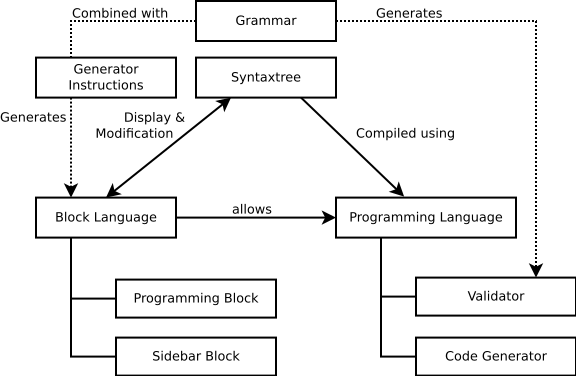
\includegraphics[width=\linewidth]{core-concepts.pdf}
  \caption{Zusammenhänge der zentralen Ressourcen}
  \label{fig:core-relations}
\end{figure}


Darüber hinaus kann durch die Speicherung eines abstrakten Syntaxbaumes der für andere Compiler typische Parsing-Vorgang entfallen. Anwender sollen Programme mit der Promotionsbegleitenden Software erstellen und editieren, nicht in einem Texteditor. Die eigentliche Aufgabe der generierten Oberfläche ist somit die Bearbeitung von Syntaxbäumen.


\section{Literaturverzeichnis}
\printbibliography[heading=none]


\end{document}
%%% Local Variables:
%%% mode: latex
%%% TeX-engine: xetex
%%% TeX-master: t
%%% TeX-command-extra-options: "-shell-escape"
%%% End:
